\documentclass[letterpaper, 12pt]{article}
\usepackage[american]{babel}
\usepackage[utf8]{inputenc}
\usepackage[citestyle=apa,style=apa,backend=biber]{biblatex}
\usepackage[margin=1in]{geometry}
\usepackage{graphicx}
\usepackage{caption}
\usepackage{float}
\usepackage{array}
\setlength\bibitemsep{2\itemsep}
\DeclareLanguageMapping{american}{american-apa}
\addbibresource{bibliography.bib}

% my version of latex does not support this character apparently..
\DeclareUnicodeCharacter{2212}{-}

\begin{document}
\begin{titlepage}
\centering
	\vspace*{5.75cm}
	{\huge\bfseries Final Report\par}
	{\large Parallelizing Machine Learning to Optimize Parameters in Genetic Algorithms\par}
	\vspace{2cm}
	Blair Urish\\
	Dan Wagner\\
	Kansas State University\\
	College of Engineering\\
	Department of Computer Science\\
	\vspace{1cm}
	Dr. Bin Liu\\
	Professor\\
	Department of Chemical Engineering\\
	\vspace{1cm}
	December 15, 2017
\end{titlepage}

\begin{abstract}
\thispagestyle{plain}
\begin{flushleft}
	It is difficult for traditional materials to have some desirable traits that often conflict with one another.  Hybrid materials are crafted to solve this, but the compounds are difficult to identify.  Using machine learning and genetic algorithms to locate the traits of these compounds has had success but is inefficient in computing power.  Thus, we have parallelized the process by distributing the work across several nodes in a master-slave relationship.  This method allowed the computation time to be spread across chunks of data, and resulted in an overall lower run time.
\end{flushleft}
\end{abstract}

\begin{flushleft}

\section*{Background Research}
Many fields require materials with properties that often conflict or trade off with one another. (\cite{Narayanan}; \cite{Ritchie}).  Examples of such properties are low density, high strength, and high flexibility.  In most cases, it is difficult or impossible for traditional materials to exhibit combinations of these properties. Therefore, it is necessary to use hybrid materials that have organic and synthetic components. However, it is difficult to identify these compounds. (\cite{Narayanan}; \cite{Wight}).\\
~\newline
Narayanan et. al. discuss two methods of identifying the components needed to create a hybrid material. The first
method discussed is known as the Reactive Force Field (ReaxFF). The authors state that ReaxFF can describe ``bond formation/dissociation, chemical reaction pathways, and transition states in a diverse class of materials.'' However, they note a major issue with ReaxFF: efficiency. ReaxFF requires a large amount of computing power to do its calculations. Many scientists require running simulations with large sample sizes to which ReaxFF does not scale. \\
~\newline
Bond order potentials (BOP) are a different approach that Narayanan et. al. believe could be significantly more
efficient than ReaxFF. They present an approach that combines Tersoff-Brenner modeling with machine learning that
allows for approximations of the attributes needed to describe the hybrid materials mentioned earlier. The goal
with this technique is to provide fairly accurate results compared with ReaxFF. The authors note that
ReaxFF will still be required for certain heterostructures like oxides. \\
~\newline
Dr. Liu's work differs from the literature in that he wishes to model platinum bonds instead of cobalt and carbon. His original solution also used different tools from the literature. It was our task to first create a program to perform this experiment using the same simulation program as the literature and then find ways to improve its runtime using parallelism. In the next section, we will discuss the methodology we used to accomplish this. 

\newpage
\section*{Methodology}
 The overall design process can be seen in the following figure.

 \begin{figure}[H]
 	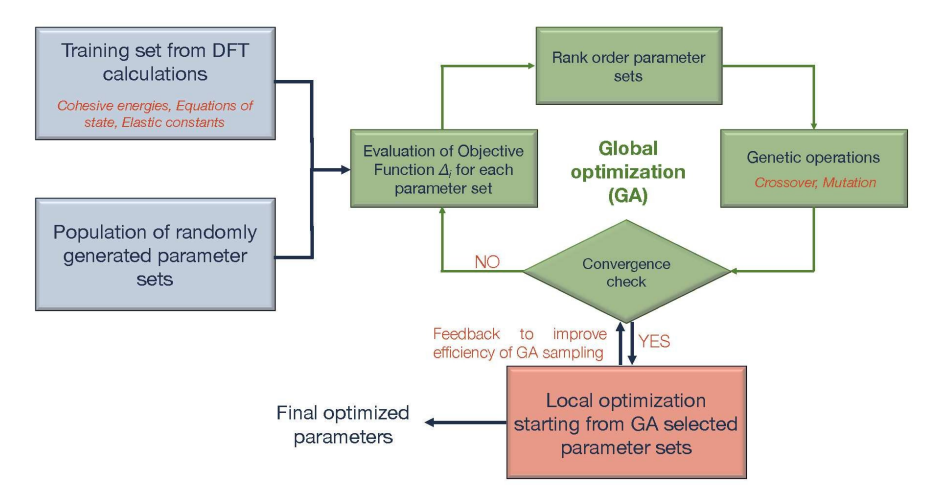
\includegraphics[width=\linewidth,height=10cm,keepaspectratio]{flowchart.png}
 	\caption[Overall Flow of Genetic Algorithm Process]{Overall Flow of Genetic Algorithm Process. Adapted from \cite{Narayanan}}
 	\label{fig:arch}
 \end{figure}

We will begin by discussing the hardware used for our project, then we will discuss the generation of parameter sets and the evaluation of the objective function for each individual first, as these
two processes work closely together. To conclude the section, we will discuss the genetic algorithm.

\subsection*{Hardware}

We will realize this solution using several nodes on the Beocat supercomputing cluster.  We restricted our usage to the Elf class nodes for benchmarking. Their specifications can be seen in the accompanying table.
~\newline

\begin{table}[ht]
	\centering
	\caption{Beocat Elf Node Specifications}
	\label{nodespecs}
	\begin{tabular}{|l|l|}
		\hline
		Processors           & 2x 8-Core Xeon E5-2690               \\ \hline
		RAM                  & 64GB                                 \\ \hline
		Hard Drives          & 1x 250GB 7200 RPM SATA               \\ \hline
		NICs                 & 4x Intel I350                        \\ \hline
		10GbE/QDR Infiniband & Mellanox Technologies MT27500 Family \\ \hline
	\end{tabular}
\end{table}

\subsection*{Individual Generation and Fitness Evaluation using LAMMPS}

Before the genetic algorithm could begin, we needed to generate random parameter sets which will function as individuals for the genetic algorithm. 
A parameter set consists of 11 parameters, each of which represent atomic traits. We were given starting values for these traits and were told to vary them by $\pm$ 25\%. 
With this information, we decided to create a C++ class to represent an individual and help keep our data organized. This class held the parameter values in a map, which mapped the parameter name to its value. 
This was chosen because it makes iterating through the parameter set extremely easy, since C++ maps support foreach loops by default. When the class was constructed, we used the new
random number generator in C++ 11 to generate values for each trait in the parameter map. Once constructed, users of the class could easily accessed the parameter map using the class's 
indexer, which we have overridden to index directly into the map. \\
~\newline
Our Individual class also held another very important value for our algorithm: the fitness. This value was calculated at the time of class construction. In order to get this value,
we had to use LAMMPS. This proved to be one of the most challenging parts of this program. LAMMPS was not a very easy program to use and much of the data that we originally received
from Dr. Liu did not work correctly and we did not know how to use it. We first tried to run LAMMPS as a standalone program from the terminal, just to get an idea of what kind of
input it expects and what kind of output it gives. We discovered that LAMMPS requires three input files. Below is a table showing each file and its purpose.

\begin{table}[ht]
	\centering
	\caption{LAMMPS Input Files}
	\label{lammpsinput}
	\begin{tabular}{|l|l|}
		\hline
		in.pt & LAMMPS configuration options. Required for every LAMMPS run \\ \hline
		data.in & Atomic geometry specification. Required for each type of atom used in simulation \\ \hline
		Pt.tersoff & Atomic parameter definition \\ \hline
	\end{tabular}
\end{table}

Our first concern when finding out how dependent LAMMPS is on these files was that file I/O was going to slow our program down greatly. LAMMPS has a C++ library, which we hoped would allow us to not even have to deal with file I/O and starting new processes at all, but unfortunately, the LAMMPS C++ library is just a simple wrapper around the normal LAMMPS executable. It will start the LAMMPS process for you, and allow you to specify an in.pt file as a string, but it does not provide a simple way to retrieve the results. LAMMPS will simply print the results as usual to the standard output stream. As far as we could tell, there was no way to directly retrieve the value we were looking for with the library.\\
~\newline
Due to the complexity and limited documentation of this library, we instead decided to just create our own code to interface with LAMMPS. Like the library, we use \texttt{popen()} to start a process. This allows us to easily gain access to its standard output stream using the standard C library functions like \texttt{fgets()}. We also piped in our in.pt file which is generated for each individual by our C++ code. This whole process was very simple to implement, unlike the LAMMPS library which made it difficult to access the output pipe and filter the output for the value we wanted. In our code, we piped the LAMMPS output into \texttt{awk} which searched for and returned the value we wanted. We don't feel that writing the code to do this in C/C++ would be significantly faster. As one will see in the performance profile, the time spent running LAMMPS itself vastly outweighs overhead from running \texttt{awk}.  \\
~\newline
As for the other files, the data.in file is shared by all LAMMPS processes because LAMMPS only needs to read from this file, not write. LAMMPS requires us to leave it on the file system anyway. In our current solution, we use two data.in files, one for each type of atomic geometry that we currently support. Adding more of these files will make the simulation more accurate, and we expect Dr. Liu to do this for his work. The last file, Pt.tersoff, is randomly generated for each individual by our program. It contains the randomly generated parameters discussed earlier. Like the data.in file, LAMMPS requires this file to be present on the file system. For our case, we simply store it in a temporary directory where it will be deleted later on. Both of these files are very small, so we do not feel that they significantly impacted our program's performance. \\
~\newline
Overall, we believe we have minimized the amount of file I/O performed in our program. One drawback to our method is that in order to add additional atomic geometry files, one has to modify the code for the Individual class, as additional LAMMPS runs need to be performed. The modifications would only involve reusing existing code, but perhaps in the future we could find a better way to handle this. 

\subsubsection*{Parallelization of Individual Generation}

After we implemented our Individual class, we discovered that it was taking approximately 15 seconds to generate each individual. This wasn't fast enough, considering we needed to have 100 individuals for our genetic algorithm. We decided to parallelize the generation of individuals, since they are not dependent on each other. This was a very straightforward process. We used OpenMP to spawn a large number of threads. Each thread will generate one individual and add it to the list of individuals that we are generating. A critical section was added to ensure two threads do not add to this list at the same time. The amount of threads that we spawn is equal to the number of cores available divided by the number of cores we permit LAMMPS to use. \\
~\newline


\subsection*{Genetic Algorithm}

~\newline
One computing node was designated as the master node, while several other nodes were the slave nodes.  OpenMP in C++ will be used in order to facilitate communication between the master and slaves. The master node received a population of randomly generated parameter sets and the training set provided.  It partitioned the population into subsets and sent the sets to slave nodes for evaluation.  The size of these partitions could vary; ideally, each node contained a chunk that fits wholly within the L3 cache. Each slave node evaluated the fitness of each individual within their subset. Then, they transfered the results back to the  master node for modification via trait crossover and mutation. The best one hundred individuals were retained for subsequent generations.  Once their fitnesses converged, and no better individuals were found, the top individual was found to be the optimized set of parameters.\\

~\newline
Our Genetics class handled the crossover of traits and the mutation of $\pm$ 33\% of the individuals.  Crossovers took two individuals and swaps their traits starting at a random trait number.  Then, the appropriate trait was found and the individuals exchanged their values for that trait.  At the end of the crossover, the two individuals' fitnesses needed to be recalculated and were done so with a call to LAMMPS.  Mutations are performed on a single individual that is randomly chosen from the dataset.  The appropriate trait was found (similarly to crossovers) and its value in the individual is recalculated.  Afterwards, its fitness is reevaluated. \\

~\newline 
This process continued until the genetic algorithm fails to return better individuals than the previous run. The most optimized individual results were be the best set of parameters for this generation. \\
~\newline
The Large-scale Atomic/Molecular Massively Parallel Simulator (LAMMPS) package was used to evaluate individuals' fitness.  This software is a classical molecular dynamics code developed by Sandia National Laboratories.  It had optimized integrations with OpenMPI, which fit into our overall design very well. \\
~\newline 
A base run time of one hour per population was established by Dr. Bin Liu.  Our implementation ran the same dataset, with the results and run times being compared for accuracy and performance.  We were expecting at least a factor of ten speedup on a single core by using OpenMP and distributing the work across several nodes.\\

\newpage
\section*{Results}
The original algorithm was quoted by Dr. Liu to have an estimated runtime of one hour per generation.  These generations contained one hundred random individuals.  Each run first generated the generation and then performed the analysis on them.  The runs used up to sixteen cores and had up to two dedicated LAMMPS cores.

\begin{figure}[H]
	\centering
	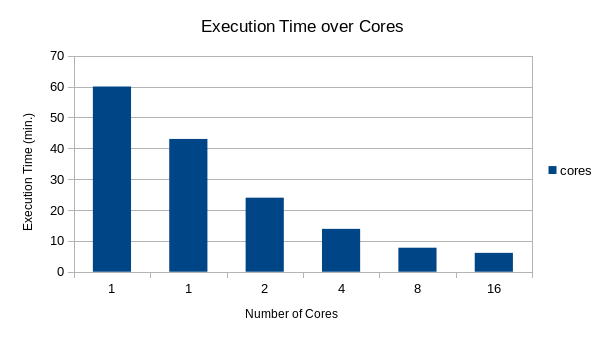
\includegraphics[width=10cm,height=10cm,keepaspectratio]{results.png}
	\caption[Run Times per Core]{Code Runtime per Number of Cores, 1 LAMMPS Core.}
	\label{fig:runtimes1core}
\end{figure}

~\newline
These runtimes can vary due to the nature of the genetic algorithm.  There was no constant number of mutated individuals, as only a random fraction of them were mutated.  The mutation process itself only occurred with a 0.1 probability.  Additionally, since both crossover and mutation must call LAMMPS to recalculate the individual's fitness, the number of iterations it takes for LAMMPS to approve of the parameters can increase runtime. \\

~\newline
A speedup of 1.4 was obtained by simply porting the codes over into C++.  As the number of cores increased, the runtime improved mostly linearly (see Table~\ref{speedups1core}).  More cores yielded additional threads to create and mutate the population with.  \\

\begin{table}[ht]
	\centering
	\caption{Speedups per Threads, 1 LAMMPS Core}
	\label{speedups1core}
	\begin{tabular}{|l|l|l|l|l|l|}
		\hline
		Threads           	& 1  & 2 & 4 & 8 & 16					\\
		\hline
		Speedup 			& 1.4 & 1.8 & 3.1 & 5.5 & 7.1			\\ 
		\hline
	\end{tabular}
\end{table}

~\newline
Next, two cores were given to LAMMPS.  This allowed us to take advantage of the built-in parallelization provided by the LAMMPS package.  Interestingly, the results were worse with two cores, rather than experiencing a speedup (Figure~\ref{fig:runtimes2cores}).

\begin{figure}[H]
	\centering
	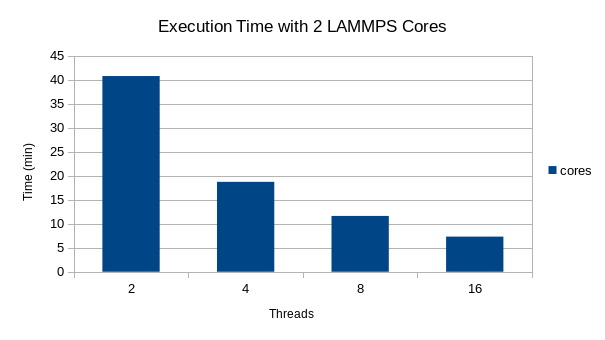
\includegraphics[width=10cm,height=10cm,keepaspectratio]{results2.png}
	\caption[Run Times per Core]{Code Runtime per Number of Cores, 2 LAMMPS Cores.}
	\label{fig:runtimes2cores}
\end{figure}

~\newline
The minimum number of cores requested per run was two due to LAMMPS' requirements. As a result, the two-core speedup is taken in reference to the hour per generation benchmark while subsequent speedups are calculated off of the two-core.  Table~\ref{speedups2core} displays this information.  Compared to Table~\ref{speedups1core}, the speedups are less and runtimes are around the same values.
\begin{table}[ht]
	\centering
	\caption{Speedups per Threads, 2 LAMMPS Cores}
	\label{speedups2core}
	\begin{tabular}{|l|l|l|l|l|}
		\hline
		Threads           	& 2 & 4 & 8 & 16					\\
		\hline
		Speedup 			& 1.5 & 2.1 & 3.5 & 5.6			\\ 
		\hline
	\end{tabular}
\end{table}

This is potentially due to less individual generation.  With more LAMMPS cores, generating individuals is faster.  However, while the generation is faster, the number of individuals being concurrently processed is cut in half.  With a single LAMMPS core and eight cores, eight copies of LAMMPS can run and yield one individual each concurrently.  When LAMMPS is given two cores and eight cores, only four copies of LAMMPS are being run, albeit faster; thus, the number of individuals concurrently created is only four.

~\newline
\begin{figure}[H]
	\centering
	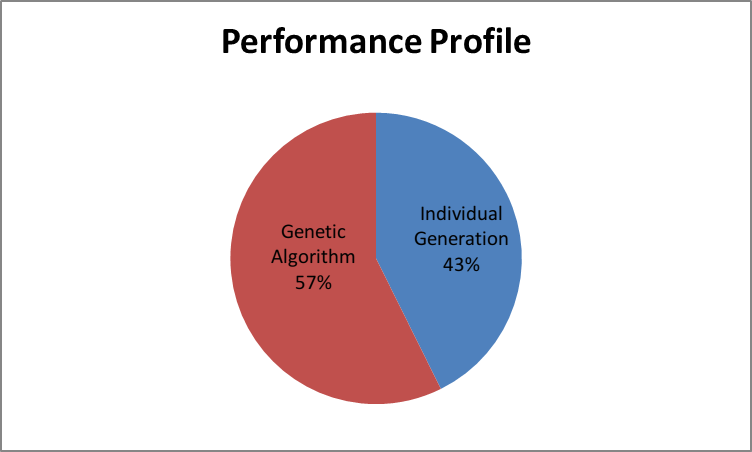
\includegraphics[width=10cm,height=10cm,keepaspectratio]{profile.png}
	\caption[Profiling]{Code Profile.}
	\label{fig:codeprofile}
\end{figure}

Figure~\ref{fig:codeprofile} demonstrates the main areas that the program spent time in.  These two sections were performing the genetic operations and initially generating the population's individuals.  The generation was generated at the beginning, while the genetic algorithm iterated multiple times before achieving convergence.  As a result, more time was spent performing crossovers and mutations than initially creating the population. \\

~\newline
\begin{figure}[H]
	\centering
	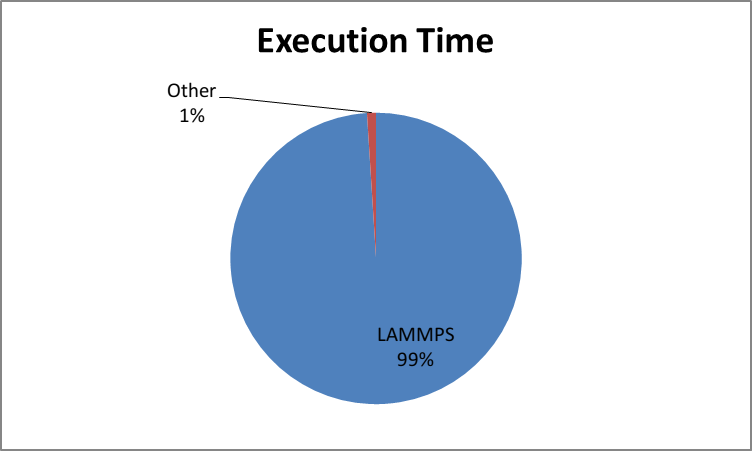
\includegraphics[width=10cm,height=10cm,keepaspectratio]{execution.png}
	\caption[Execution]{Code Execution Profile.}
	\label{fig:execprofile}
\end{figure}

Figure~\ref{fig:execprofile} shows the amount of time spent in LAMMPS versus the rest of the program.  LAMMPS overwhelmingly takes the most time to complete its operations, while the main C++ program takes very little time.  LAMMPS computations dominate our code when evaluating the fitness of individuals, which happens at the beginning, and during genetic operations.  The C++ program, outside of LAMMPS, spends little time comparatively to sort the individuals, determine the probabilities of genetic operations, and print the results. \\

\newpage
\section*{Conclusions}
We have parallelized the process of optimizing hybrid material properties in genetic algorithms.  A global single-population master-slave approach  divided up the population into subsets of individuals and then passed them to slave nodes.  Slaves operated on their data with LAMMPS and evaluated the fitness of each individual.  These results were sent back to the master node who performed genetic operations on them.  On average, the solution experienced a linear speedup with the number of cores.

\section*{Future Work}
Future work will include implementing the master-slave genetic algorithm using OpenMPI and C++ with an interface into LAMMPS.  The software will be benchmarked and checked for accuracy.
\newpage
\printbibliography

\end{flushleft}
\end{document}
